\documentclass{article}

% Language setting
% Replace `english' with e.g. `spanish' to change the document language
\usepackage[english]{babel}

% Set page size and margins
% Replace `letterpaper' with `a4paper' for UK/EU standard size
\usepackage[letterpaper,top=2cm,bottom=2cm,left=3cm,right=3cm,marginparwidth=1.75cm]{geometry}

% Useful packages
\usepackage{amsmath}
\usepackage{graphicx}
\usepackage[colorlinks=true, allcolors=blue]{hyperref}

% custom
\usepackage{caption}
\usepackage{float}

\title{Aprendizado de Máquina \\ Trabalho Prático 1}
\author{Luís Felipe Ramos Ferreira \\ 2019022553}

\begin{document}
\maketitle

\section{Introdução}

O Trabalho Prático 1 da disciplina de Aprendizado de Máquina teve como tema a criação de uma rede neuronal para classificação de dígitos escritos a mão, mais especificamente o conhecido conjunto de dados MNIST. Os objetivos do trabalho envolviam analisar como o modelo da rede neuronal iria variar na convergência do erro empírico conforme são modificadas diferentes variáveis de configuração da rede, como a taxa de aprendizado, a quantidade de neurônios na camada oculta e diferentes algoritmos de cálculo de gradiente.

\section{Implementação}

A linguagem escolhida para o desenvolvimento do trabalho foi Python (versão 3.10), devida a sua grande variedade de bibliotecas úteis para ciência de dados e aprendizado de máquina. A modelagem da rede neuronal foi feita com o uso da API keras disponibilizada na biblioteca TensorFlow, uma vez que se tratava de uma ferramenta extremamente completa para todos os objetivos do trabalho que permitia grande flexibilidade na modelagem da rede.

Para organizar o ambiente, que englobava várias bibliotecas diferentes, foi utilizado o gerenciador de pacotes Anaconda, o que tornou muito mais fácil trabalhar com os pacotes de ciência de dados citados.

\section{Experimentos}

Os experimentos foram realizados sobre uma subparte da base de dados MNIST, disponibilizados no enunciado do trabalho. Essa parte possui um total de 5000 instâncias, que foram divididas em conjunto de treino (90\%) e conjunto de teste (10\%).

Conforme especificado, foram testados e comparados os resultados da rede neuronal na classificação dos dígitos para diferentes parâmetros de modelagem. Mais especificamente, todas as permutações das seguintes configurações foram utilizadas:

\begin{itemize}
    \item Número de neurônios na camada oculta
        \begin{itemize}
            \item 25
            \item 50
            \item 100
        \end{itemize}
    \item Algoritmo de cálculo de gradiente 
        \begin{itemize}
            \item \textit{Gradient Descent} (O gradiente é calculado após cada época, neste caso, 5000 entradas)
            \item \textit{Stochastic Gradient Descent} (O gradiente é calculado após cada entrada)
            \item \textit{Mini batch} (O gradiente é calculado após um certo número de entradas, neste caso, 10 e 50)
        \end{itemize}
    \item Taxa de aprendizado 
        \begin{itemize}
            \item 0.5
            \item 1.0
            \item 10.0
        \end{itemize}
\end{itemize}

Para fins de analisar também como o número de épocas de treino afeta o modelo, todas as configurações possíveis descritas acima foram utilizadas em modelos que treinaram por 10, 50 e 100 épocas.

O resultado obtido para cada umas das 108 configurações foi armazenado em um arquivo \textit{JSON}, de modo que sua leitura e manipulação fosse facilitada, e assim bibliotecas de análise de dados como Pandas pudessem ser utilizadas para interpretar
como se comportou cada parametrização do modelo durante o treino.

\section{Análise dos resultados de teste}

De maneira geral, os dados gerados deixaram muito claro quais as configurações que permitiam uma boa e uma má performance do modelo. As duas tabelas a seguir mostram os parâmetros das 10 configurações que obtiveram o menor valor de acurácia no conjunto de treino, assim como as 10 configurações com o maior valor de acurácia.

\begin{table}[H]
    \centering
        \captionsetup{labelformat=empty} 
        \caption{10 piores desempenhos}
        \begin{tabular}{| c c c c c |}
        \hline
        Épocas & Tamanho da camada oculta & Tamanho do lote & Taxa de aprendizado & Acurácia \\
        \hline
            100 &  25 &    1 & 10.0 & 0.098 \\
            100 &  50 &    1 & 10.0 & 0.098 \\
            100 & 100 &    1 & 10.0 & 0.098 \\
            10 &  50 &    1 & 10.0 & 0.108 \\
            10 &  25 &    1 & 10.0 & 0.110 \\
            50 &  50 &    1 & 10.0 & 0.120 \\
            50 &  25 &    1 & 10.0 & 0.128 \\
            50 & 100 &    1 & 10.0 & 0.170 \\
            10 &  50 & 4500 & 10.0 & 0.176 \\
            10 & 100 &    1 & 10.0 & 0.182 \\
        \hline
        \end{tabular}
\end{table}

\begin{table}[H]
    \centering
        \captionsetup{labelformat=empty} 
        \caption{10 melhores desempenhos}
        \begin{tabular}{| c c c c c |}
        \hline
        Épocas & Tamanho da camada oculta & Tamanho do lote & Taxa de aprendizado & Acurácia \\
        \hline
            50 & 100 & 10 & 1.0 & 0.946 \\
            50 & 100 & 10 & 0.5 & 0.944 \\
            50 & 100 & 50 & 1.0 & 0.942 \\
            100 & 100 & 10 & 0.5 & 0.942 \\
            10 & 100 & 10 & 1.0 & 0.940 \\
            100 & 100 & 10 & 1.0 & 0.940 \\
            100 & 100 & 50 & 1.0 & 0.940 \\
            10 &  50 & 10 & 0.5 & 0.938 \\
            50 &  50 & 10 & 0.5 & 0.938 \\
            10 & 100 & 50 & 1.0 & 0.936 \\
        \hline
        \end{tabular}
\end{table}

Em primeiro lugar, evidencia-se o fato de que todos os 10 piores valores de acurácia obtidos nos dados de treino ocorreram em modelos com uma taxa de aprendizado igual a 10. Isso indica que uma taxa de aprendizado alta não é uma boa opção para o treino de uma rede neuronal, devido ao fato de que uma alta taxa leva a uma grande quantidade de oscilações durante o treino, gerando alta divergência do erro empírico e, consequentemente, um modelo de baixíssima performance.

Outro fato relevante a se notar é o tamanho dos lotes que geraram os piores resultados. Dentre os 10 piores modelos criados, 9 utilizavam ou o algoritmo \textit{Stochastic Gradient Descent} (tamanho de lote igual a 1). Isso, no entanto, não quer dizer que o uso dessa abordagem seja ruim. O \textit{SGD} é um algoritmo que pode sim gerar bons resultados e ter uma boa performance. O detalhe principal que o levou a aparecer tantas vezes no topo dos piores modelos é a taxa de aprendizado alta, como citada anteriormente. Como a cada entrada os pesos da rede serão alterados, a alta taxa de aprendizado torna ainda mais grave a divergência do erro empírico e causa ainda mais confusão.

Por outro lado, os 10 modelos com os melhores desempenhos em acurácia demonstram que uma taxa de aprendizado equilibrada é um importante fator para um bom resultado. Todos os modelos na tabela contêm taxas de 0.5 ou 1.0. Pode-se notar também que prevalecem entre os melhores modelos tamanhos de lote igual a 10 ou 50, ou seja, o uso do algoritmo Mini batch se mostrou o mais performático na construção da rede neuronal. Isso é esperado, dado que a intuição do algoritmo de gradiente Mini batch é justamente evitar valores extremos para atualização dos pesos da rede, o que aumenta o poder de generalização da rede.

Por fim, nota-se que 8 entre os 10 modelos com melhor resultado possuem 100 neurônios na camada oculta. Tal fato confirma as hipóteses de que, com mais neurônios, o modelo irá aprender a identificar mais padrões e terá mais poder de generalização. No entanto, deve-se ter cuidado com esse parâmetro da rede, uma vez que números muito altos de neurônios nas camadas ocultas podem gerar problemas relacionados a alta variãncia do modelo gerado.

Em resumo, nota-se que as configurações da rede impactam diretamente em sua performance, e esses parâmetros devem ser estimados com cuidado e suas escolhas feitas considerando cada detalhe necessário para ter um modelo capaz de generalizar bem os dados ao final do treinamento.

\subsection{Trade-off entre número de unidades da camada oculta e algoritmo de cálculo de gradiente}

Ao analisar os diferentes desempenhos da rede neuronal de acordo com a variação entre o número de unidades da camada oculta e o algoritmo de gradiente utilizado, podemos inferir diretamente que o aumento do número de neurônios
causa um impacto positivo  no desempenho do modelo. Tal inferência faz sentido, uma vez que com uma rede com mais neurônios, mais informações podem ser extraídas e dessa maneira de melhor forma o modelo poderá generalizar sobre
dados ainda não vistos. No entanto, fica claro que um abuso desse hiperparâmetro é algo que pode levar a \textit{overfitting}.

Nos gráficos abaixo, podemos ver a variação da acurácia do modelo nos dados de teste em função da variação do número de unidades na camada oculta, para cada um dos algoritmo de cálculo de gradiente propostos.

\begin{figure}[htbp]
    \centering
    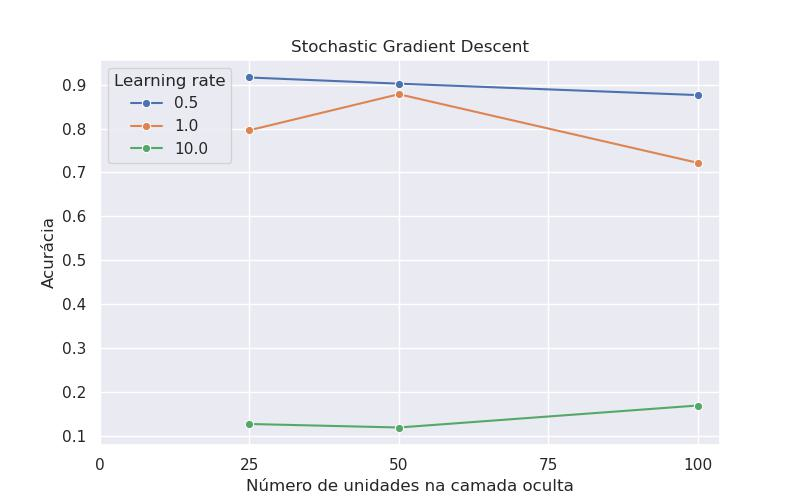
\includegraphics[width=0.8\textwidth]{images/tradeoff/SGD.jpg}
    \caption{Acurácia por número de neurônios para o algoritmo \textit{Stochastic Gradient Descent}}
\end{figure}

\begin{figure}[htbp]
    \centering
    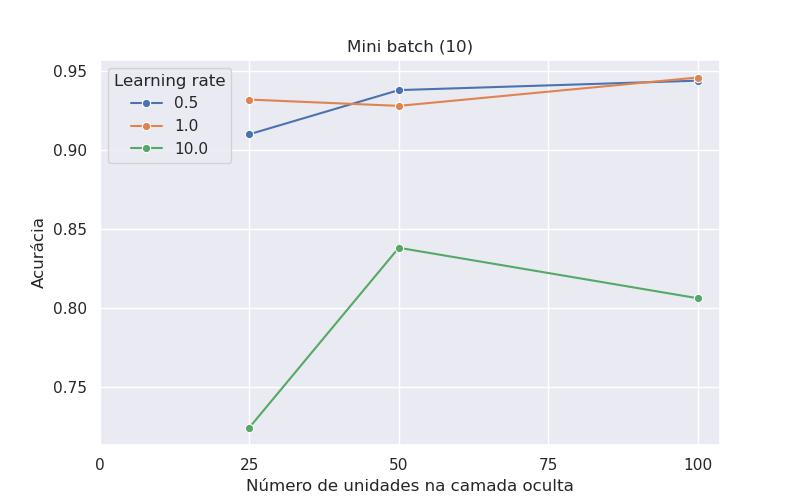
\includegraphics[width=0.8\textwidth]{images/tradeoff/MB10.jpg}
    \caption{Acurácia por número de neurônios para o algoritmo \textit{Mini batch} (10)}
\end{figure}

\begin{figure}[htbp]
    \centering
    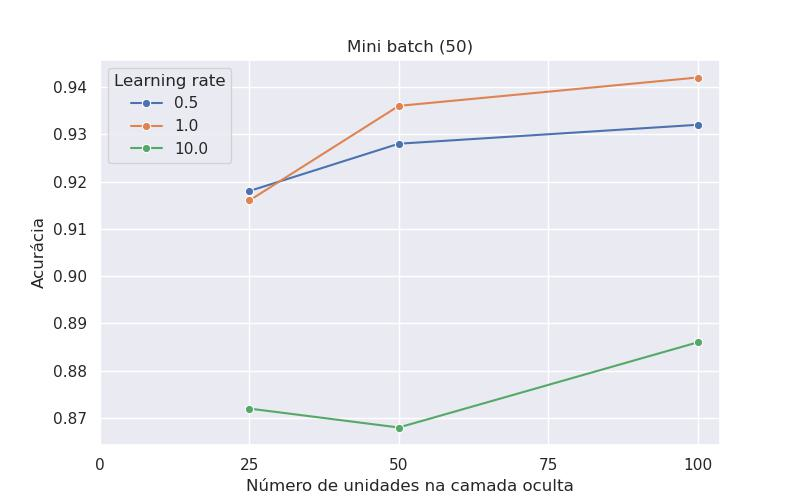
\includegraphics[width=0.8\textwidth]{images/tradeoff/MB50.jpg}
    \caption{Acurácia por número de neurônios para o algoritmo \textit{Mini batch} (50)}
\end{figure}

\begin{figure}[htbp]
    \centering
    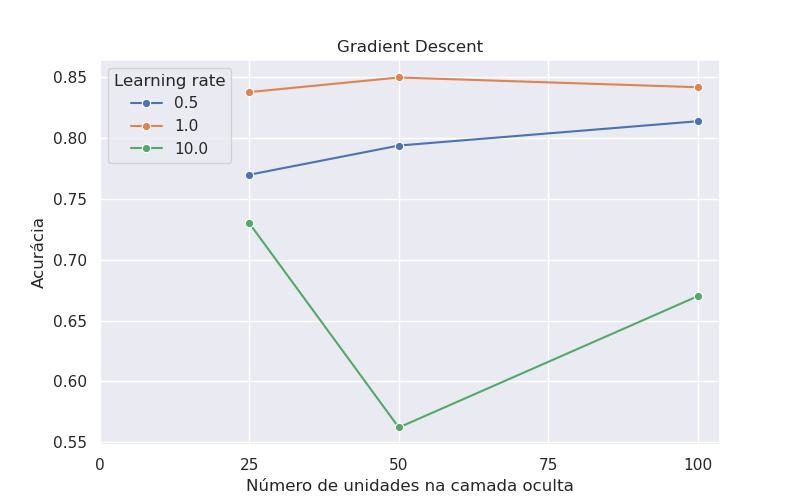
\includegraphics[width=0.8\textwidth]{images/tradeoff/GD.jpg}
    \caption{Acurácia por número de neurônios para o algoritmo \textit{Gradient Descent}}
\end{figure}


FALAR MAIS AQUI

\section{Convergência do erro empírico}

Durante o treinamento das redes neuronais propostas, o histórico do erro empírico pode ser armazenado para análise de sua convergência, considerando cada configuração de rede proposta.

\end{document}